\chapter{Gravity, Free Fall, and Newton's Theorem}

Gravity enters this course already carrying a double burden. It is one force among others, but it is also the force that seems to know something about geometry. Susskind therefore begins with a deliberate narrowing of scope. We are not yet doing the full general theory of relativity. We are doing Newtonian gravity, but we are doing it in a way that will later make the passage to general relativity feel motivated rather than abrupt: first the Newtonian language of forces and vectors, then the cancellation of mass in gravitational motion, then the full inverse-square law, and finally the vector calculus that explains why spherical gravitating bodies behave as if all their mass were concentrated at a point.

\paragraph{Source note.} These companion notes follow Leonard Susskind's first general relativity lecture and preserve its order of argument. This draft was prepared with support from LazyingArt LLC and Video2Book.

\section{Gravity as a Special Force and Why We Start With Newton}

Susskind opens by saying, in effect, that gravity is unusual. Electric and magnetic forces do not behave like it, and somehow gravity is tied to the geometry of space and time. But precisely because of that, he does not begin with curved spacetime. He begins with Newton.

\begin{definition}
An inertial frame is a coordinate system, equipped with clocks, in which a force-free test object moves with uniform velocity and therefore has zero acceleration.
\end{definition}

This is the lecture's first piece of discipline. Before we speak about gravity, we must know what we mean by force, acceleration, coordinates, and vectors. The preserved frame below catches the board at the moment when Susskind has written only the bare scalar-looking equation \(F=ma\). The transcript makes clear, however, that he is already speaking of a three-dimensional vector equation.

\begin{figure}
\centering

\includegraphics[width=0.62\textwidth]{lecture_01_figure_02.png}
\caption{The lecture begins from the stripped-down Newtonian law. The board still shows the scalar handwriting \(F=ma\), but the spoken lecture already treats it as the vector equation \(\vec F = m\vec a\).}
\end{figure}

Thus we write
\begin{align}
\vec F &= m\vec a, \\
F_i &= m a_i = m\ddot x_i, \qquad i=1,2,3.
\end{align}
The mass \(m\) is a scalar. In Newtonian physics it is conserved: it may be redistributed from one place to another, but it is not itself a directional object.

A particle has coordinates \(x_1,x_2,x_3\), which together form the position vector
\begin{equation}
\vec r=(x_1,x_2,x_3).
\end{equation}
Its first time derivative is velocity and its second time derivative is acceleration:
\begin{equation}
v_i=\dot x_i, \qquad a_i=\ddot x_i.
\end{equation}
This is the quiet mathematical framework within which the special feature of gravity will soon appear. If the gravitational force carries the same mass that already sits in Newton's law, then that mass may cancel, and when it cancels the motion stops depending on the nature of the falling object.

\section{Galileo's Flat-Earth Gravity and the First Equivalence-Principle Lesson}

Now the lecture deliberately steps backward from Newton to Galileo. This is not antiquarianism. Galileo isolates the simplest approximation in which gravity reveals what is peculiar about it.

In the flat-Earth approximation two simplifications hold at once. First, the direction of gravity is everywhere the same: downward. Second, its magnitude does not depend on height. If we choose the \(x_2\)-axis to be vertical and take upward to be positive, then the gravitational force has only one nonzero component:
\begin{equation}
F_2=-mg.
\end{equation}
The minus sign merely says that the force points downward. Here \(g\) is the near-surface gravitational acceleration. On Earth it is about \(10\,\mathrm{m/s^2}\); on the Moon it is smaller, on Jupiter larger. What matters in the present argument is that for a given planet it does not depend on the mass of the falling body.

Combining Galileo's force law with Newton's equation gives the first decisive cancellation:
\begin{align}
F_2 &= m\ddot x_2, \\
m\ddot x_2 &= -mg, \\
\ddot x_2 &= -g.
\end{align}
This is the first serious mathematical signal of the equivalence principle in the lecture. The acceleration of free fall is independent of the mass of the object. Heavy bodies and light bodies obey the same equation of motion. However Galileo performed the experiment, whether from a tower or on an inclined plane, this is the content of the result: absent air resistance, different masses fall alike.

The crucial point is that this is not true for generic forces. Electric forces couple to charge, not mass. Gravity is special because its force is proportional to the same mass that Newton's law then multiplies by the acceleration. The mass cancels, and with it goes any dependence of the motion on the identity of the falling body.

\subsection{Question \& Answer}

Why can a freely falling cloud fail to detect gravity even though gravity is present?

Take a diffuse cloud of particles and let them all go in the same uniform gravitational field. Some particles may be heavy, some light, some large, some small. None of that matters. Every particle obeys \(\ddot x_2=-g\). Therefore every particle falls in exactly the same way.

The consequence is stronger than the slogan ``all bodies fall alike.'' The cloud does not deform. Neighboring particles keep the same relative separation. If the cloud had been held together by struts, those struts would feel no stress from the gravitational field itself, because all parts of the structure share the same motion. In the flat-Earth approximation, gravity produces no internal stretching, no compression, and no shear.

That is why Susskind says that free fall is locally indistinguishable from being far away from all gravitating bodies. The point is not that one cannot tell the difference between standing on the Earth and falling. Of course one can. The point is subtler: within a self-contained falling system, and without using an external reference such as the floor, one cannot detect the gravitational field by internal mechanical measurements.

The student questions in the lecture push this further. Is the effect optically detectable? Suppose the particles in the cloud carry lasers. The answer is still no, because the relative distances do not change. Is the peculiar feeling of stepping off a building evidence of gravitational acceleration? Again no. That feeling comes from the disappearance of the support forces that normally act on the bottoms of our feet. In Susskind's phrase, what we ordinarily feel is not falling but \emph{not} falling.

This is the lecture's first version of the equivalence principle: in a perfectly uniform gravitational field, free fall erases gravity locally.

\section{Newton's Inverse-Square Force: From Magnitude to Direction}

The flat-Earth approximation has now done its work. The lecture turns to Newton's full force law. Every object in the universe exerts a gravitational force on every other object. Start with two masses, a lighter mass \(m\) and a heavier mass \(M\). The forces are attractive, equal, and opposite.

The board first presents the law as a statement about magnitude, not yet about direction. In the preserved frame the denominator is written as \(R^2\); we keep that equation visible because it is legible on the board, but in the polished formulas below we normalize the notation to \(r=|\vec r|\).

\begin{figure}
\centering

\includegraphics[width=0.72\textwidth]{lecture_01_figure_03.png}
\caption{The lecture first writes Newton's law as a statement about force magnitude. The point-source sketch labeled \(M\) prepares the immediate transition to vector form.}
\end{figure}

On the board one sees
\begin{equation}
F=\frac{mMG}{R^2}.
\end{equation}
In cleaned notation we write
\begin{equation}
F=\frac{GmM}{r^2},
\end{equation}
where \(G\) is Newton's constant,
\begin{equation}
G\approx 6.7\times 10^{-11}\,\mathrm{N\,m^2/kg^2}.
\end{equation}
The lecture pauses over the smallness of this number. Gravity is weak. That is not merely rhetoric. For two \(1\,\mathrm{kg}\) masses separated by \(1\,\mathrm{m}\),
\begin{equation}
F = G \approx 6.7\times 10^{-11}\,\mathrm N.
\end{equation}
A bit of electrostatic charge or a modest magnet easily beats that. Gravity dominates ordinary life only because the Earth is so heavy.

There is another special feature here as well. Electric forces may attract or repel. Gravitational forces, in Newton's theory, are always attractive.

Now Susskind sharpens the scalar law into a vector law. Put the heavy mass \(M\) at the origin and let \(\vec r\) point from \(M\) to the lighter particle \(m\). Then the force on \(m\) must point along the radial direction, but opposite to \(\vec r\). Introducing the unit vector
\begin{equation}
\hat r=\frac{\vec r}{r},
\end{equation}
we obtain
\begin{equation}
\vec F
=
-\frac{GmM}{r^2}\hat r
=
-\frac{GmM}{r^3}\vec r.
\end{equation}
The extra factor of \(r\) downstairs is exactly what keeps the magnitude at \(1/r^2\) while inserting the direction.

\begin{figure}
\centering
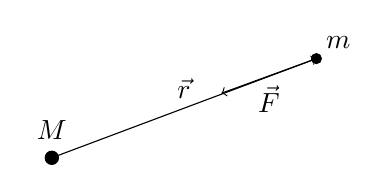
\begin{tikzpicture}[scale=1.05]
\draw[fill=black] (0,0) circle (0.08);
\node[above] at (0,0.1) {$M$};
\draw[fill=black] (3.2,1.2) circle (0.06);
\node[above right] at (3.2,1.2) {$m$};
\draw[->] (0,0) -- (3.2,1.2) node[midway, above] {$\vec r$};
\draw[->] (3.2,1.2) -- (2.05,0.78) node[midway, below] {$\vec F$};
\end{tikzpicture}
\caption{Clean reconstruction of the geometry behind the vector law. The radial vector points from the source mass \(M\) to the test mass \(m\), while the force points inward, opposite to \(\vec r\).}
\end{figure}

\subsection{Question \& Answer}

\paragraph{Equal forces, unequal accelerations.}
If the force on the Earth due to a falling body is equal and opposite to the force on the body due to the Earth, why does the Earth hardly accelerate at all?

Because equality of forces is not equality of accelerations. Newton's equation says
\[
\vec a=\frac{\vec F}{m}.
\]
For the same force, the larger mass has the smaller acceleration. The Earth and the falling body exert equal forces on one another, but the Earth's enormous mass suppresses its acceleration.

\paragraph{Why inverse square?}
The lecture's historical motivation runs through Kepler. For circular motion of radius \(r\) and angular frequency \(\omega\), the inward acceleration is
\begin{equation}
a_{\mathrm{circ}}=\omega^2 r.
\end{equation}
If the force per unit mass behaves as \(f(r)\propto 1/r^2\), then
\begin{equation}
\omega^2 r \propto \frac{1}{r^2},
\qquad\text{so}\qquad
\omega^2\propto \frac{1}{r^3}.
\end{equation}
Since \(T=2\pi/\omega\), we obtain
\begin{equation}
T^2\propto r^3.
\end{equation}
This is Kepler's law relating period and orbital radius. In the lecture this is not meant as a full historical reconstruction, but as the right Newtonian clue: Kepler's law points strongly toward the inverse-square force, and the inverse-square force is then the law that extends correctly beyond perfect circles to the ellipse.

\paragraph{What if the bodies get too close?}
The lecture also inserts a caution. When bodies touch, or even come sufficiently close, gravity is no longer the whole story. Electrostatic, atomic, and nuclear forces enter. Newton's inverse-square law is the right long-range gravitational law, not a complete short-distance theory of matter.

\section{From Two Bodies to Many Bodies}

Now we pass from one pair of gravitating bodies to a whole assembly of particles. Newtonian gravity works pairwise, but the total force on a given particle is the vector sum of all the pairwise forces exerted by the others. Susskind pauses to remark that this superposition rule is not logically forced by the idea of force itself; it is a fact about Newtonian gravity.

The available board witness for this part of the lecture is weak but useful. It catches the many-body formula in the middle of a live correction, just as the sign convention is being discussed and the board is already being erased.

\begin{figure}
\centering

\includegraphics[width=0.74\textwidth]{lecture_01_figure_04.png}
\caption{Documentary witness for the many-body discussion. The board is already being erased and the sign convention is being corrected live, so the final notes immediately replace the unstable blackboard notation by a clean standard form.}
\end{figure}

Let \(\vec r_i\) be the position of the \(i\)-th particle. If we define the vector from particle \(i\) to particle \(j\) by \(\vec r_j-\vec r_i\), then the clean Newtonian force law is
\begin{equation}
\vec F_i
=
\sum_{j\ne i}
G\,m_i m_j\,
\frac{\vec r_j-\vec r_i}{|\vec r_j-\vec r_i|^3}.
\end{equation}
This is the simplest way to encode attraction without importing the lecture's temporary sign ambiguity. The student objection in the lecture is exactly that one may put the minus sign in front or absorb it into the choice of whether the vector points from \(i\) to \(j\) or from \(j\) to \(i\). Once the convention is fixed, the formula is fixed.

Now combine this with Newton's equation for the same particle:
\begin{align}
\vec F_i &= m_i\vec a_i, \\
m_i\vec a_i
&=
\sum_{j\ne i}
G\,m_i m_j\,
\frac{\vec r_j-\vec r_i}{|\vec r_j-\vec r_i|^3}.
\end{align}
The mass \(m_i\) cancels:
\begin{equation}
\vec a_i
=
\sum_{j\ne i}
G\,m_j\,
\frac{\vec r_j-\vec r_i}{|\vec r_j-\vec r_i|^3}.
\end{equation}
Once again the motion of the particle we are tracking does not depend on its own mass. It depends on the masses of all the other particles, but not on its own. This is the same structural fact we already saw in the flat-Earth problem, now stated for the general Newtonian field.

The lecture also inserts an important warning here. This formula tells us the instantaneous force if we know the positions of all the particles. Once the entire system is allowed to evolve, every particle changes the motion of every other particle, and the full dynamics quickly becomes a complicated many-body problem. That complication is real, but it is not the point of the present lecture. The present point is the persistence of mass-independence in the motion of a test object.

\section{Tidal Forces as the Repair to Uniform Free Fall}

At this point the lecture returns to the earlier statement about free fall and tightens it. In the flat-Earth approximation we said that a freely falling object does not detect gravity internally. That statement was deliberately a little too strong. It is true only for a perfectly uniform field.

Once the force depends on distance from the source, not all parts of an extended body accelerate in exactly the same way. If a very tall body falls feet-first toward the Earth, the feet are closer to the Earth than the head, so the lower part experiences a stronger acceleration. The body is stretched vertically. In differential language, nearby parts separated by \(\delta \vec x\) experience different accelerations because
\begin{equation}
\delta \vec a \approx \vec g(\vec x+\delta \vec x)-\vec g(\vec x)
\end{equation}
is no longer negligible.

There is a second effect. If the same extended body lies horizontally, then its left and right ends are pulled toward the Earth's center along slightly different directions. The field is radial, so those forces are not parallel. The body is therefore squeezed horizontally even if the magnitudes of the forces are nearly the same. In the lecture this becomes the vivid picture of the absurdly tall man who is stretched in one orientation and compressed in another.

These are tidal forces. They are real. They are not an artifact of coordinates. They arise because the Newtonian gravitational field varies in both magnitude and direction from point to point.

\subsection{Question \& Answer}

If free fall hides gravity, why do sufficiently large falling bodies get stretched and squeezed?

Because free fall hides only the common part of the acceleration. If the field were perfectly uniform, every part of the body would share the same motion and nothing internal would reveal gravity. But a real gravitational field is not uniform. Different parts of the body sample different values and different directions of the field, and those differences are exactly what produce stress and strain.

So the lecture keeps two statements at once. A sufficiently small freely falling object does not notice gravity, because the gradient of the field across its size is negligible. A sufficiently large freely falling object does notice gravity, because that gradient is not negligible. Then one part is pulled a little harder than another, or one part is pulled in a slightly different direction than another, and the body is stretched or squeezed.

This is also why the forces are called \emph{tidal}. The Moon exerts such forces on the Earth. The solid Earth is comparatively rigid, but the oceans are not. The water layer is therefore slightly stretched along the Earth--Moon line and squeezed in the transverse directions, producing the familiar tidal bulges.

\section{The Gravitational Field}

Only after this correction does Susskind define the gravitational field. The definition is operational. We imagine adding one more particle, a very light particle, light enough that it does not appreciably influence the motion of the others. This extra particle is the test particle.

\begin{definition}
The gravitational field at a point \(\vec x\) is the acceleration of a sufficiently light test particle placed at \(\vec x\).
\end{definition}

This definition is tailored to the special property of gravity. Since the force is proportional to the mass of the test particle, the ratio of force to mass is independent of which test particle we use. We may therefore think directly in terms of acceleration rather than force. The field is the vector acceleration assigned to each point in space.

If the source masses are at positions \(\vec r_j\), a clean Newtonian expression is
\begin{equation}
\vec g(\vec x)
=
\sum_j G\,m_j\,
\frac{\vec r_j-\vec x}{|\vec r_j-\vec x|^3}.
\end{equation}
The lecture temporarily denotes this acceleration by \(\vec A\). We keep \(\vec g\) for the gravitational field itself and reserve \(\vec A\) for the generic vector field used in the vector-calculus discussion after the break.

The field is a vector field. It has magnitude and direction, it depends on position, and if the source masses move it depends on time as well. That is the right place for the lecture to pause. Once the field has been laid out over space, we need the mathematics that describes how such a field varies from point to point.

\section{Divergence, Gauss's Theorem, and Newton's Theorem}

After the break Susskind says openly that we now need a little fancy mathematics. The first object is a generic vector field \(\vec A(\vec x)\), not yet necessarily the gravitational field. We want a scalar quantity that measures whether the field is locally spreading out from a point or converging into it.

The board below preserves the lecture's definition.

\begin{figure}
\centering

\includegraphics[width=0.84\textwidth]{lecture_01_figure_05.png}
\caption{The board formula for divergence. The key distinction is between the vector field \(\vec A\) and the scalar quantity \(\nabla\cdot\vec A\).}
\end{figure}

In cleaned notation we write
\begin{equation}
\nabla\cdot\vec A
=
\partial_x A_x+\partial_y A_y+\partial_z A_z
=
\frac{\partial A_x}{\partial x}
+\frac{\partial A_y}{\partial y}
+\frac{\partial A_z}{\partial z}.
\end{equation}
The lecture is careful about the point that this is a scalar, not a vector. The arrows drawn on the other board are the field \(\vec A\) itself. The divergence is the scalar quantity extracted from the spatial derivatives of its components.

To make this intuitive, the lecture turns to water flow. We imagine a shallow lake of fixed depth, or more generally an incompressible fluid whose density is fixed. Water pumped in from below creates a local source, so the velocity field spreads outward and has positive divergence. Water removed from below creates a sink, so the field converges inward and has negative divergence. The lecture later notes that one could complicate the analogy by allowing compression or thinning, but for pedagogy it keeps the picture simple: fixed depth, fixed density, visible source and sink language.

The accompanying arrow-field sketch is preserved below.

\begin{figure}
\centering

\includegraphics[width=0.50\textwidth]{lecture_01_figure_06.png}
\caption{Schematic field used in the lecture to explain local divergence. The point is to compare the amount of flow entering and leaving a small control region.}
\end{figure}

\begin{figure}
\centering
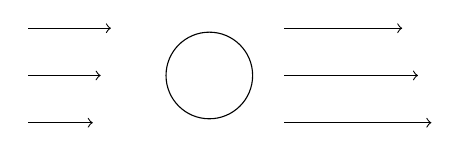
\begin{tikzpicture}[scale=1.0]
\draw[->] (-2.3,1.0) -- (-1.25,1.0);
\draw[->] (-2.3,0.4) -- (-1.38,0.4);
\draw[->] (-2.3,-0.2) -- (-1.48,-0.2);

\draw[->] (0.95,1.0) -- (2.45,1.0);
\draw[->] (0.95,0.4) -- (2.65,0.4);
\draw[->] (0.95,-0.2) -- (2.82,-0.2);

\draw (0.0,0.4) circle (0.55);
\end{tikzpicture}
\caption{Reconstruction of the control-region picture described in the lecture. More field leaves the small circle on the right than enters from the left, so the region has positive divergence.}
\end{figure}

The second tool is Gauss's theorem, which ties local source strength to total flux through a boundary.

\begin{theorem}[Gauss's theorem]
For a vector field \(\vec A\),
\begin{equation}
\int_V (\nabla\cdot\vec A)\,dV
=
\oint_{\partial V} A_\perp\,d\sigma
=
\oint_{\partial V} \vec A\cdot \hat n\,d\sigma.
\end{equation}
\end{theorem}

The meaning is direct. The integral on the left adds up all sources and sinks inside the region \(V\). The integral on the right adds up the net outward flow through the boundary \(\partial V\). Only the normal component matters; motion tangent to the boundary slides along it and contributes no outward flux.

This is the theorem the lecture has been building toward. We now apply it to a spherically symmetric source of divergence concentrated inside some finite sphere. Let the total enclosed divergence be
\begin{equation}
Q=\int_V (\nabla\cdot\vec A)\,dV.
\end{equation}
If we surround that source by a larger sphere of radius \(r\), then \(Q\) is independent of the radius of the larger sphere, provided only that the larger sphere encloses the whole source region.

By spherical symmetry, the field outside must be radial and its magnitude must be constant over the Gaussian sphere. Therefore the flux integral collapses to
\begin{align}
Q
&=
\oint_{\partial V} A_\perp\,d\sigma
=
A(r)\oint_{\partial V} d\sigma \\
&= 4\pi r^2\,A(r).
\end{align}
Hence
\begin{equation}
A(r)=\frac{Q}{4\pi r^2},
\qquad
\vec A(r)=\frac{Q}{4\pi r^2}\hat r.
\end{equation}
This is the lecture's clean derivation of a \(1/r^2\) field from spherical symmetry and Gauss's theorem. It is here that Susskind briefly says ``four-thirds \(\pi r^2\)'' and immediately corrects it. Only the corrected surface area \(4\pi r^2\) belongs in the notes.

Now gravity reenters. A positive source in the water analogy gives an outward field. Real Newtonian gravity points inward. So the gravitational analog is a negative source, or a convergence. For a point mass \(M\),
\begin{equation}
\vec g(r)=-\frac{GM}{r^2}\hat r.
\end{equation}
The lecture emphasizes that this is only a mathematical analogy. Space is not literally a fluid. But the analogy is useful because it explains why a point source naturally produces a \(1/r^2\) field.

This brings us to Newton's theorem.

\begin{proposition}[Newton's theorem]
Outside a spherically symmetric mass distribution, the gravitational field is exactly the same as that of a point mass with the same total mass concentrated at the center.
\end{proposition}

This is not a small convenience. It is what makes planetary gravity tractable. The exterior field of a spherical planet does not care whether the mass is concentrated at the center, spread out smoothly, denser in the middle, or denser near the surface. Outside the body, only the total mass matters.

\begin{figure}
\centering
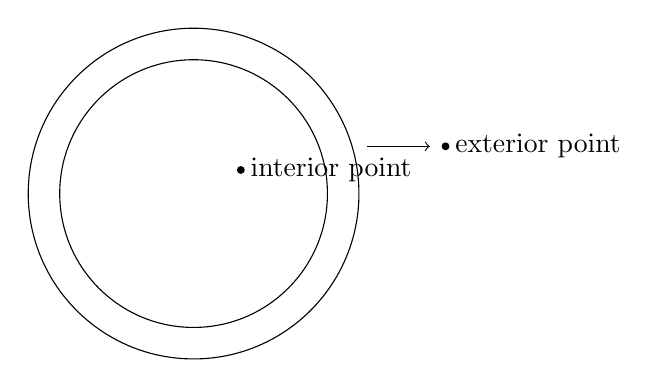
\begin{tikzpicture}[scale=1.0]
\draw (0,0) circle (1.7);
\draw (0,0) circle (2.1);
\fill (0.6,0.3) circle (0.05);
\node[right] at (0.6,0.3) {interior point};
\fill (3.2,0.6) circle (0.05);
\node[right] at (3.2,0.6) {exterior point};
\draw[->] (2.2,0.6) -- (3.0,0.6);
\end{tikzpicture}
\caption{A spherical shell. Outside the shell, the field is the same as that of a point mass at the center. Inside the shell, the field vanishes.}
\end{figure}

\subsection{Question \& Answer}

Why is the field outside a spherical body point-mass-like, while the field inside a spherical shell vanishes?

Outside the body, the answer is Gauss plus symmetry. A Gaussian sphere enclosing the entire spherically symmetric source sees only the total enclosed mass. The flux is therefore fixed. Since the field has the same magnitude everywhere on that sphere and points radially, the only possible exterior field is the \(1/r^2\) field of a point mass with that same total mass.

Inside a hollow spherical shell, the answer is sharper still. A Gaussian surface entirely inside the shell encloses no source at all. Therefore the enclosed divergence is zero, and the net flux through the Gaussian surface is zero. But by symmetry there is no distinguished interior direction. The only field compatible with zero enclosed source and full spherical symmetry is
\[
\vec g_{\text{inside shell}}=0.
\]

The lecture also insists on the corresponding limitation. This is an exterior theorem. Once we go inside a gravitating body, we are asking a different question. In the mine shaft thought experiment the field near the center of the Earth is certainly not what it would be if the entire Earth's mass were concentrated at the center. The exterior theorem does not survive unchanged at interior points.

Susskind is right to linger here. This theorem is not just elegant; it is the remarkable piece of luck that made Newtonian celestial mechanics workable.

\section{Summary}

The lecture begins with the most elementary Newtonian equation and ends with the shell theorem, but the movement is carefully staged. First we learn why gravity is special: its force is proportional to the same mass that appears in Newton's law, so in a uniform field the mass cancels and free fall becomes universal. Then we leave the flat-Earth approximation, write Newton's inverse-square law, sharpen it into vector form, and generalize it to many bodies. The motion of a test particle still ignores its own mass, which leads naturally to the gravitational field.

Only then do we stop and repair the earlier slogan. A real gravitational field varies from place to place, so large freely falling bodies are stretched and squeezed by tidal forces. After the break the lecture introduces divergence and Gauss's theorem, and these become the machinery that explains why spherical symmetry produces a \(1/r^2\) law and why spherical shells are so remarkable.

That is the real payoff of Lecture 1. Already within Newtonian gravity, the mathematics begins to organize itself in a way that points beyond force law and toward geometry.